% ============================================================
% NVIDIA Certified Associate - Generative AI LLMs (NCA-GENL) Slide Deck
% Custom Navasena Dark Beamer Theme
% Compiler: xelatex
% ============================================================
\documentclass[aspectratio=169,t]{beamer}

% ---- Fonts (xelatex) ----------------------------------------
\usepackage{fontspec}
\usepackage[sfdefault]{FiraSans}

% ---- Core packages ------------------------------------------
\usepackage{graphicx}
\usepackage{tikz}
\usetikzlibrary{positioning, shapes.geometric, arrows.meta, calc}
\usepackage{pgfplots}
\pgfplotsset{compat=1.18}
\usepackage{pgf-pie}
\usepackage{amsmath}
\usepackage{booktabs}
\usepackage{colortbl}
\usepackage{xcolor}
\usepackage{pifont}

% ============================================================
% COLOR PALETTE (Navasena dark theme)
% ============================================================
\definecolor{nvbg}{HTML}{1A1A2E}
\definecolor{nvdark}{HTML}{1A1A2E}
\definecolor{nvcard}{HTML}{2D2D44}
\definecolor{nvgreen}{HTML}{76B900}
\definecolor{nvlightgreen}{HTML}{A3D944}
\definecolor{nvwhite}{HTML}{FFFFFF}
\definecolor{nvgray}{HTML}{AAAACC}
\definecolor{nvdarkcard}{HTML}{23233A}
\definecolor{nvred}{HTML}{EF5350}
\definecolor{nvorange}{HTML}{FF6F00}
\definecolor{nvblue}{HTML}{42A5F5}

% ============================================================
% BEAMER THEME — NAVASENA DARK
% ============================================================
\usetheme{default}
\usecolortheme{default}

\setbeamercolor{background canvas}{bg=nvbg}
\setbeamercolor{normal text}{fg=nvwhite}
\setbeamercolor{frametitle}{fg=nvwhite, bg=nvbg}
\setbeamercolor{framesubtitle}{fg=nvgray, bg=nvbg}
\setbeamercolor{title}{fg=nvgreen}
\setbeamercolor{author}{fg=nvgray}
\setbeamercolor{date}{fg=nvgray}
\setbeamercolor{item}{fg=nvgreen}
\setbeamercolor{subitem}{fg=nvlightgreen}
\setbeamercolor{subsubitem}{fg=nvgray}
\setbeamercolor{block title}{fg=nvwhite, bg=nvcard}
\setbeamercolor{block body}{fg=nvwhite, bg=nvcard}

\setbeamertemplate{footline}{%
  \hbox{%
    \begin{beamercolorbox}[wd=\paperwidth,ht=2ex,dp=0.6ex,leftskip=2em]{author in head/foot}%
      \color{nvgray}\small\textbf{NVIDIA NCA-GENL Certification} \hfill \insertframenumber\,/\,\inserttotalframenumber
    \end{beamercolorbox}%
  }%
}
\setbeamertemplate{navigation symbols}{}

% ---- Global vertical compaction (fit dense slides) ----------
\setbeamerfont{frametitle}{size=\large,series=\bfseries}
\setbeamerfont{framesubtitle}{size=\scriptsize}
\addtobeamertemplate{frametitle}{}{\vspace{-0.55em}}
\setlength{\leftmargini}{1.3em}
\setlength{\leftmarginii}{1.0em}
% tighten itemize/enumerate vertical rhythm globally
\makeatletter
\def\@listi{\leftmargin\leftmargini \topsep 2pt \parsep 0pt \itemsep 2pt}
\let\@listI\@listi
\def\@listii{\leftmargin\leftmarginii \topsep 1pt \parsep 0pt \itemsep 1pt}
\makeatother
% compact display-math spacing
\setlength{\abovedisplayskip}{3pt}
\setlength{\belowdisplayskip}{3pt}
\setlength{\abovedisplayshortskip}{1pt}
\setlength{\belowdisplayshortskip}{1pt}

% ============================================================
% CUSTOM COMMANDS
% ============================================================
% \acttitle{N}{Title}{Subtitle}
\newcommand{\acttitle}[3]{%
  \begin{frame}[plain]
    \vspace{1.5cm}
    \begin{center}
      {\color{nvgreen}\Huge\bfseries Act #1}\\[1.2em]
      {\color{nvwhite}\Huge #2}\\[0.8em]
      {\color{nvgray}\Large #3}
    \end{center}
  \end{frame}%
}
% \takeaway{...}  — green one-line summary box
\newcommand{\takeaway}[1]{%
  \vspace{0.1em}
  \begin{beamercolorbox}[rounded=true,shadow=false,sep=5pt]{block body}
    \centering\footnotesize\color{nvlightgreen}#1
  \end{beamercolorbox}%
}
% \certnote{Domain}{teks} — small certification-domain callout
\newcommand{\certnote}[2]{%
  \vspace{0.1em}
  \begin{beamercolorbox}[rounded=true,shadow=false,sep=4pt]{block body}
    {\scriptsize\color{nvblue}\textbf{Sertifikasi NCA-GENL --- #1:}}\,
    {\scriptsize\color{nvgray}#2}
  \end{beamercolorbox}%
}

\title{NVIDIA Certified Associate --- Generative AI LLMs}
\subtitle{Panduan Lengkap \& Strategi Ujian (Exam Code: NCA-GENL)}
\author{Navasena AI}
\date{}

% ============================================================
\begin{document}

% ── Slide 1 — Title ───────────────────────────────────────
\begin{frame}[plain]
  \vspace{1.0cm}
  \begin{center}
    {\color{nvgreen}\Huge\bfseries NVIDIA Certified Associate}\\[0.9em]
    {\color{nvwhite}\Huge\bfseries Generative AI \& Large Language Models}\\[0.5em]
    {\color{nvgray}\Large Panduan Lengkap Kurikulum, Domain, dan Strategi Lulus Ujian NCA-GENL}\\[1.6em]

    
\begin{tikzpicture}[scale=0.85, every node/.style={transform shape},
        b/.style={draw=nvgreen, fill=nvcard, rounded corners=6pt, text=white, font=\small, minimum width=2.0cm, minimum height=0.9cm, align=center}]
      \node[b] (g) {AI\\Knowledge};
      \node[b, right=0.5cm of g] (s) {Data\\Analysis};
      \node[b, right=0.5cm of s] (f) {Experi-\\mentation};
      \node[b, right=0.5cm of f, draw=nvblue] (r) {Software\\Dev};
      \node[b, right=0.5cm of r, draw=nvorange] (a) {Trustworthy\\AI};
      \draw[->,thick,color=nvgreen] (g)--(s);
      \draw[->,thick,color=nvgreen] (s)--(f);
      \draw[->,thick,color=nvgreen] (f)--(r);
      \draw[->,thick,color=nvorange] (r)--(a);
    \end{tikzpicture}

    \vspace{0.8em}
    {\color{nvgray}\small Waktu: 60 Menit $\cdot$ 50--60 Soal Pilihan Ganda $\cdot$ Online Proctored $\cdot$ Navasena AI 2026}
  \end{center}
\end{frame}

% ── Slide 2 — Peta perjalanan ─────────────────────────────
\begin{frame}{Peta Perjalanan Kurikulum Sertifikasi}
  \framesubtitle{Distribusi materi ujian berdasarkan lima domain resmi blueprint NVIDIA}
  \begin{center}
  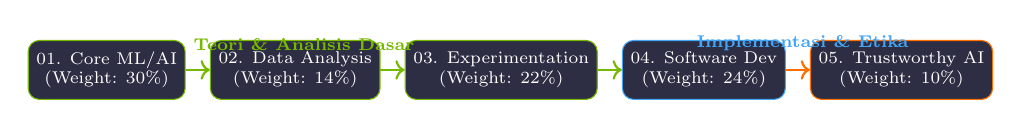
\begin{tikzpicture}[scale=0.88, every node/.style={transform shape},
      s/.style={draw=nvgreen, fill=nvcard, rounded corners=4pt, text=white, font=\scriptsize, minimum width=2.2cm, minimum height=0.85cm, align=center},
      t/.style={draw=nvblue, fill=nvcard, rounded corners=4pt, text=white, font=\scriptsize, minimum width=2.2cm, minimum height=0.85cm, align=center}]
    \node[s] (a) {01. Core ML/AI\\(Weight: 30\%)};
    \node[s, right=0.35cm of a] (b) {02. Data Analysis\\(Weight: 14\%)};
    \node[s, right=0.35cm of b] (c) {03. Experimentation\\(Weight: 22\%)};
    \node[t, right=0.35cm of c] (d) {04. Software Dev\\(Weight: 24\%)};
    \node[t, draw=nvorange, right=0.35cm of d] (e) {05. Trustworthy AI\\(Weight: 10\%)};
    \draw[->,thick,color=nvgreen] (a)--(b); \draw[->,thick,color=nvgreen] (b)--(c);
    \draw[->,thick,color=nvgreen] (c)--(d); \draw[->,thick,color=nvorange] (d)--(e);
    \node[text=nvgreen, font=\scriptsize\bfseries, above=0.15cm] at ($(a)!0.5!(c)$) {Teori \& Analisis Dasar};
    \node[text=nvblue, font=\scriptsize\bfseries, above=0.15cm] at ($(d)!0.5!(e)$) {Implementasi \& Etika};
  \end{tikzpicture}
  \end{center}
  \takeaway{Sertifikasi NCA-GENL menguji pemahaman konsep fundamental AI ($\sim$70\% platform-agnostic) dan ekosistem NVIDIA ($\sim$30\% tool-specific).}
\end{frame}

% ============================================================
\acttitle{1}{Overview \& Format Ujian}{Mengenal format dasar, target audiens, dan pembagian bobot nilai}

% ── Apa itu Sertifikasi NCA-GENL? ─────────────────────────
\begin{frame}{Apa itu Sertifikasi NCA-GENL?}
  \framesubtitle{Validasi kredensial profesional untuk Generative AI dan Large Language Models}
  \begin{columns}[T]
    \begin{column}{0.55\textwidth}
      \begin{itemize}\footnotesize
        \item \textbf{NVIDIA Certified Associate}: Validasi keahlian tingkat pemula-menengah dalam merancang dan men-deploy aplikasi Generative AI.
        \item \textbf{Fokus Kurikulum}: Menguji kemampuan integrasi LLM, prompt engineering, optimasi inferensi, dan etika kecerdasan buatan.
        \item \textbf{Target Audiens}: AI DevOps engineers, data scientists, software engineers, dan solution architects.
        \item \textbf{Prasyarat}: Pemahaman dasar tentang generative AI dan LLM (direkomendasikan juga dasar pemrograman Python dan machine learning).
      \end{itemize}
    \end{column}
    \begin{column}{0.42\textwidth}
      \begin{center}
        
\begin{tikzpicture}[scale=0.9, every node/.style={transform shape}]
          \draw[nvgreen, thick, fill=nvdarkcard] (0,0) circle (1.5cm);
          \node[align=center, text=nvwhite, font=\bfseries\small] at (0,0) {NVIDIA\\Certified\\Associate};
          \draw[nvblue, thick] (0,0) circle (1.65cm);
          \node[text=nvlightgreen, font=\tiny, below=1.9cm] at (0,0) {Generative AI \& LLM Associate};
        \end{tikzpicture}
      \end{center}
    \end{column}
  \end{columns}
  \takeaway{Sertifikasi ini sangat bernilai untuk memvalidasi pemahaman praktis mengenai cara kerja dan penyajian model AI di industri.}
\end{frame}

% ── Mekanisme & Format Ujian ──────────────────────────────
\begin{frame}{Mekanisme \& Format Ujian}
  \framesubtitle{Detail administratif dan teknis pelaksanaan ujian sertifikasi}
  \begin{center}
  \renewcommand{\arraystretch}{1.02}{\footnotesize\setlength{\tabcolsep}{10pt}
  \begin{tabular}{@{}p{0.3\linewidth}p{0.6\linewidth}@{}}
    \toprule \rowcolor{nvcard!50}
    \textbf{Komponen Ujian} & \textbf{Detail Spesifikasi} \\ \midrule
    Nama Ujian & NVIDIA Certified Associate -- Generative AI LLMs \\
    Exam Code & NCA-GENL \\
    Level & Associate (entry-level) \\
    Jumlah Soal & 50--60 soal pilihan ganda \\
    Durasi Waktu & 60 Menit ($\sim$60--72 detik per soal) \\
    Biaya & USD 125 \\
    Validitas & 2 tahun (recert via ujian ulang) \\
    Bahasa & Inggris \\
    Metode Pengawasan & Online proctored (webcam) \\
    Skor Kelulusan & Tidak dipublikasikan oleh NVIDIA \\
    \bottomrule
  \end{tabular}}
  \end{center}
  \takeaway{NVIDIA tidak mempublikasikan skor kelulusan resmi --- targetkan penguasaan merata di semua domain, dan kelola waktu (flag soal sulit, lanjut dulu).}
\end{frame}

% ── Pembagian Domain Resmi ───────────────────────────────
\begin{frame}{Pembagian Lima Domain Ujian}
  \framesubtitle{Pembobotan resmi untuk menentukan fokus belajar}
  \begin{columns}[T]
    \begin{column}{0.55\textwidth}
      \begin{itemize}\footnotesize
        \item \textbf{Core ML/AI Knowledge (30\%)}: Porsi terbesar, menguji teori dasar ML/DL dan arsitektur model transformer.
        \item \textbf{Software Development (24\%)}: Menguji penulisan kode Python untuk RAG, spaCy, NumPy, dan deployment.
        \item \textbf{Experimentation (22\%)}: Berfokus pada evaluasi model, optimasi inferensi, dan fine-tuning.
        \item \textbf{Data Analysis \& Viz (14\%)}: Menguji EDA, preprocessing data, data mining, dan visualisasi.
        \item \textbf{Trustworthy AI (10\%)}: Menguji keamanan model, privasi data (GDPR/UU-PDP), dan bias.
      \end{itemize}
    \end{column}
    \begin{column}{0.42\textwidth}
      \begin{center}
        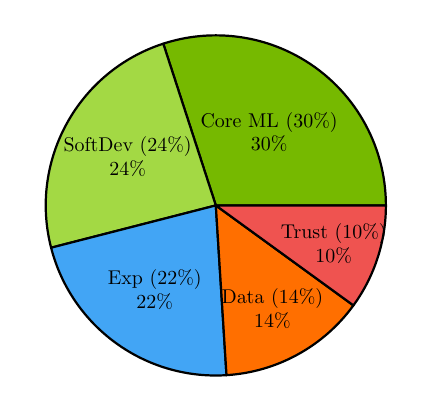
\begin{tikzpicture}[scale=0.72, every node/.style={transform shape}]
          \pie[color={nvgreen, nvlightgreen, nvblue, nvorange, nvred}, text=inside, sum=100]{
            30/Core ML (30\%),
            24/SoftDev (24\%),
            22/Exp (22\%),
            14/Data (14\%),
            10/Trust (10\%)
          }
        \end{tikzpicture}
      \end{center}
    \end{column}
  \end{columns}
  \certnote{Penting}{Hampir setengah dari nilai ujian (54\%) bertumpu pada Software Development dan Core ML/AI Knowledge.}
\end{frame}

% ============================================================
\acttitle{2}{Domain 1: Core ML \& AI Knowledge}{Pemahaman arsitektur model, mekanisme attention, dan dasar-dasar LLM (30\%)}

% ── Machine Learning Fundamentals ─────────────────────────
\begin{frame}{Dasar-Dasar Machine Learning}
  \framesubtitle{Tipe pembelajaran dan alur kerja pemodelan tradisional}
  \begin{columns}[T]
    \begin{column}{0.52\textwidth}
      \begin{itemize}\footnotesize
        \item \textbf{Supervised Learning}: Belajar dari data berlabel. Contoh: Klasifikasi dan Regresi.
        \item \textbf{Unsupervised Learning}: Menemukan pola tersembunyi pada data tanpa label. Contoh: Clustering (K-Means) dan Reduksi Dimensi.
        \item \textbf{Self-Supervised Learning}: Model membuat label sendiri dari data mentah. Sangat krusial untuk pre-training LLM (next token prediction).
        \item \textbf{Reinforcement Learning}: Belajar melalui agen yang berinteraksi dengan lingkungan via reward/penalty. Dasar dari RLHF.
      \end{itemize}
    \end{column}
    \begin{column}{0.45\textwidth}
      \begin{center}
      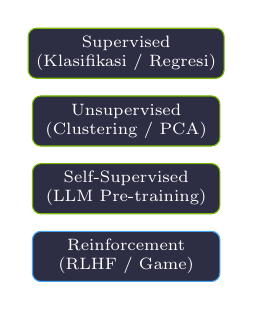
\begin{tikzpicture}[scale=0.85, every node/.style={transform shape},
          n/.style={draw=nvgreen, fill=nvcard, rounded corners=3pt, text=white, font=\scriptsize, minimum width=2.8cm, minimum height=0.6cm, align=center}]
        \node[n] (a) {Supervised\\(Klasifikasi / Regresi)};
        \node[n, below=0.25cm of a] (b) {Unsupervised\\(Clustering / PCA)};
        \node[n, below=0.25cm of b] (c) {Self-Supervised\\(LLM Pre-training)};
        \node[n, below=0.25cm of c, draw=nvblue] (d) {Reinforcement\\(RLHF / Game)};
      \end{tikzpicture}
      \end{center}
    \end{column}
  \end{columns}
  \certnote{Core ML/AI Knowledge}{Pahami perbedaan mendasar tipe pembelajaran di atas beserta contoh algoritmanya (regresi linear, logistic, random forest, XGBoost).}
\end{frame}

% ── Deep Learning & Neural Networks ───────────────────────
\begin{frame}{Deep Learning \& Neural Networks}
  \framesubtitle{Komponen penyusun jaringan saraf tiruan dan proses latihannya}
  \begin{columns}[T]
    \begin{column}{0.58\textwidth}
      \begin{itemize}\footnotesize
        \item Jaringan saraf terdiri dari \textbf{Input Layer}, \textbf{Hidden Layers}, dan \textbf{Output Layer} dengan bobot (weights) dan bias yang dapat dipelajari.
        \item \textbf{Activation Functions} (Non-linearitas):
          \begin{itemize}\scriptsize
            \item \textbf{ReLU}: $f(x) = \max(0, x)$ --- Paling populer di hidden layers.
            \item \textbf{GELU}: Dipakai secara luas di model Transformer (BERT, GPT).
            \item \textbf{Sigmoid/Softmax}: Dipakai di output layer untuk probabilitas klasifikasi.
          \end{itemize}
        \item \textbf{Backpropagation}: Algoritma pencarian gradien fungsi loss terhadap bobot menggunakan chain rule untuk memperbarui parameter model.
        \item \textbf{Optimizers}: Algoritma pembaruan bobot (SGD, Adam, AdamW untuk regulasi bobot pada Transformer).
      \end{itemize}
    \end{column}
    \begin{column}{0.38\textwidth}
      \begin{center}
      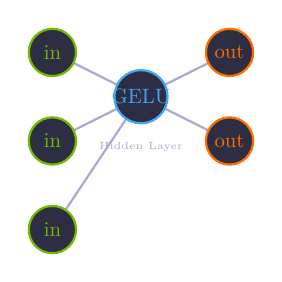
\begin{tikzpicture}[scale=0.75, every node/.style={transform shape}]
        \draw[thick, nvgray] (0,1.5) -- (1.5,0.75) -- (3,1.5);
        \draw[thick, nvgray] (0,0) -- (1.5,0.75) -- (3,0);
        \draw[thick, nvgray] (0,-1.5) -- (1.5,0.75);
        \draw[thick, nvgreen, fill=nvcard] (0,1.5) circle (0.4cm) node {in};
        \draw[thick, nvgreen, fill=nvcard] (0,0) circle (0.4cm) node {in};
        \draw[thick, nvgreen, fill=nvcard] (0,-1.5) circle (0.4cm) node {in};
        \draw[thick, nvblue, fill=nvcard] (1.5,0.75) circle (0.45cm) node {GELU};
        \draw[thick, nvorange, fill=nvcard] (3,1.5) circle (0.4cm) node {out};
        \draw[thick, nvorange, fill=nvcard] (3,0) circle (0.4cm) node {out};
        \node[text=nvgray, font=\tiny, below=0.1cm] at (1.5,0.2) {Hidden Layer};
      \end{tikzpicture}
      \end{center}
    \end{column}
  \end{columns}
  \takeaway{Backpropagation menghitung gradien secara mundur, sementara Optimizer menentukan arah pembaruan bobot berdasarkan gradien tersebut.}
\end{frame}

% ── Arsitektur Transformer & Attention ───────────────────
\begin{frame}{Arsitektur Transformer \& Attention}
  \framesubtitle{Revolusi pemrosesan paralel menggantikan arsitektur RNN/LSTM}
  \begin{columns}[T]
    \begin{column}{0.54\textwidth}
      \begin{itemize}\scriptsize
        \item \textbf{Kelemahan RNN/LSTM}: Proses sekuensial (token-by-token) lambat, hilangnya memori jangka panjang (vanishing gradient).
        \item \textbf{Mekanisme Self-Attention}: Mengizinkan model melihat semua token serentak dan menentukan hubungan antar token.
        \item Tiap token menghasilkan proyeksi vektor Query ($Q$), Key ($K$), dan Value ($V$).
        \item \textbf{Rumus Skala Dot-Product Attention}:
          $$\text{Attention}(Q, K, V) = \text{softmax}\left(\frac{QK^T}{\sqrt{d_k}}\right)V$$
        \item \textbf{Masked Attention}: Menutup token masa depan pada decoder agar tidak bocor (cheating) saat latihan.
      \end{itemize}
    \end{column}
    \begin{column}{0.42\textwidth}
      \begin{center}
      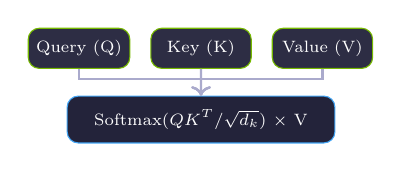
\begin{tikzpicture}[scale=0.85, every node/.style={transform shape},
          n/.style={draw=nvgreen, fill=nvcard, rounded corners=4pt, text=nvwhite, font=\scriptsize, minimum width=1.5cm, minimum height=0.6cm, align=center}]
        \node[n] (q) {Query (Q)};
        \node[n, right=0.3cm of q] (k) {Key (K)};
        \node[n, right=0.3cm of k] (v) {Value (V)};
        \node[draw=nvblue, fill=nvdarkcard, rounded corners=4pt, text=nvwhite, font=\scriptsize,
              below=0.4cm of k, minimum width=4cm, minimum height=0.7cm, align=center] (att) {Softmax($QK^T / \sqrt{d_k}$) $\times$ V};
        \draw[->,thick,nvgray] (q.south) -- +(0,-0.15) -| (att.north);
        \draw[->,thick,nvgray] (k.south) -- (att.north);
        \draw[->,thick,nvgray] (v.south) -- +(0,-0.15) -| (att.north);
      \end{tikzpicture}
      \end{center}
    \end{column}
  \end{columns}
  \certnote{Core ML/AI Knowledge}{Pahami peran pembagi $\sqrt{d_k}$ (mencegah nilai dot product yang terlalu besar dan menjamin gradien softmax tetap stabil).}
\end{frame}

% ── Positional Encoding ──────────────────────────────────
\begin{frame}{Positional Encoding}
  \framesubtitle{Memberikan informasi urutan/posisi kata pada proses perhatian paralel}
  \begin{itemize}\small
    \item \textbf{Kenapa Butuh?}: Self-attention bersifat \emph{permutation-invariant} (mengacak urutan kalimat menghasilkan representasi yang sama).
    \item \textbf{Sinusoidal (Original Transformer)}: Menggunakan fungsi sinus dan kosinus pada frekuensi berbeda. Statis/tidak dilatih.
    \item \textbf{Learned Positional Embeddings}: Menggunakan vektor posisi yang ikut dilatih bersama bobot model (dipakai di BERT, GPT-3).
    \item[] \textbf{\color{nvlightgreen}Model Modern:}
    \item \textbf{RoPE (Rotary Position Embedding)}: Memutar representasi query dan key menggunakan matriks rotasi. Mendukung ekstrapolasi panjang konteks yang lebih baik (dipakai di LLaMA, Qwen).
    \item \textbf{ALiBi (Attention with Linear Biases)}: Menambahkan bias penalti linier berdasarkan jarak token langsung pada skor attention.
  \end{itemize}
  \takeaway{RoPE dan ALiBi adalah standar untuk model bahasa modern karena unggul dalam menangani kalibrasi konteks yang sangat panjang.}
\end{frame}

% ── Tipe Model: Encoder vs Decoder ────────────────────────
\begin{frame}{Tipe Arsitektur Transformer}
  \framesubtitle{Tiga orientasi arsitektur berdasarkan blok yang digunakan}
  \begin{center}
  \renewcommand{\arraystretch}{1.25}{\footnotesize\setlength{\tabcolsep}{8pt}
  \begin{tabular}{@{}p{0.20\linewidth}p{0.25\linewidth}p{0.20\linewidth}p{0.22\linewidth}@{}}
    \toprule \rowcolor{nvcard!50}
    \textbf{Tipe Arsitektur} & \textbf{Mekanisme Attention} & \textbf{Contoh Model} & \textbf{Kegunaan Utama} \\ \midrule
    \textbf{Encoder-Only} & Bidirectional (dua arah) & BERT, RoBERTa & Klasifikasi teks, NER, ekstraksi embeddings \\
    \textbf{Decoder-Only} & Masked Causal (satu arah) & GPT, LLaMA, Mistral & Generasi teks, Chatbots \\
    \textbf{Encoder-Decoder} & Campuran + Cross-Attention & T5, BART & Penerjemahan bahasa, Ringkasan dokumen \\
    \bottomrule
  \end{tabular}}
  \end{center}
  \takeaway{BERT (Encoder) melihat masa lalu dan masa depan secara bersamaan. GPT (Decoder) hanya melihat masa lalu untuk menebak kata berikutnya.}
\end{frame}

% ── Tokenization Strategies ──────────────────────────────
\begin{frame}{Strategi Tokenisasi}
  \framesubtitle{Cara memecah string teks menjadi unit numerik (token)}
  \begin{columns}[T]
    \begin{column}{0.55\textwidth}
      \begin{itemize}\small
        \item \textbf{BPE (Byte-Pair Encoding)}: Memulai dari tingkat karakter, menggabungkan pasangan byte/karakter yang paling sering muncul berulang kali. (Dipakai di GPT).
        \item \textbf{WordPiece}: Mirip BPE, namun memilih pasangan gabungan berdasarkan maksimalisasi \emph{likelihood} dari data bahasa. (Dipakai di BERT).
        \item \textbf{SentencePiece}: Mengatasi keterbatasan spasi pada bahasa non-Latin. Memperlakukan teks sebagai aliran byte mentah (spasi diganti $\_$).
      \end{itemize}
    \end{column}
    \begin{column}{0.42\textwidth}
      \begin{center}
      \begin{beamercolorbox}[rounded=true,shadow=false,sep=8pt]{block body}
        {\footnotesize\color{nvlightgreen}\textbf{Gotcha Ujian:}}
        \vspace{0.3em}
        {\scriptsize\color{nvwhite}Tokenisasi $\neq$ Embedding!\\
        $\bullet$ \textbf{Tokenisasi}: Memecah string menjadi token/ID integer.\\
        $\bullet$ \textbf{Embedding}: Mengubah ID integer tersebut menjadi vektor bernilai kontinu (dense vector).}
      \end{beamercolorbox}
      \end{center}
    \end{column}
  \end{columns}
  \takeaway{Subword tokenization (BPE/WordPiece) memecahkan masalah kata di luar kamus (\emph{Out-Of-Vocabulary} atau OOV) secara efisien.}
\end{frame}

% ============================================================
\acttitle{3}{Domain 2: Data Analysis \& Visualization}{Eksplorasi data, metrik performa statistik, dan ekosistem RAPIDS (14\%)}

% ── Preprocessing & Outliers ──────────────────────────────
\begin{frame}{Eksplorasi \& Pembersihan Data}
  \framesubtitle{Langkah awal menjaga kualitas data latih model Generative AI}
  \begin{itemize}\footnotesize
    \item \textbf{Missing Values Imputation}:
      \begin{itemize}\scriptsize
        \item \emph{MCAR (Missing Completely at Random)}: Baris data bisa langsung dihapus tanpa memicu bias.
        \item \emph{Imputasi Sentral}: Mengisi nilai kosong dengan Mean/Median (data numerik) atau Mode (data kategori).
        \item \emph{Forward/Backward Fill}: Mengisi dengan baris sebelum/sesudah (sangat ideal untuk data runtun waktu/time-series).
      \end{itemize}
    \item \textbf{Deteksi \& Penanganan Pencilan (Outliers)}:
      \begin{itemize}\scriptsize
        \item \emph{Z-Score}: Data dianggap pencilan jika nilainya di luar $\pm 3$ standar deviasi.
        \item \emph{IQR (Interquartile Range)}: Batas pencilan adalah di luar range $[Q1 - 1.5 \times IQR]$ hingga $[Q3 + 1.5 \times IQR]$.
        \item \emph{Winsorization}: Mengganti nilai ekstrem pencilan dengan nilai persentil tertentu (misal persentil ke-1 atau ke-99).
      \end{itemize}
  \end{itemize}
  \takeaway{Pembersihan data wajib dilakukan sebelum pelatihan. Jaringan saraf sangat sensitif terhadap rentang nilai ekstrem dan data kosong.}
\end{frame}

% ── NLP Vectorization Pipelines ───────────────────────────
\begin{frame}{Metode Vektorisasi Teks NLP}
  \framesubtitle{Evolusi dari representasi kata yang statis hingga dinamis berbasis konteks}
  \begin{center}
  \renewcommand{\arraystretch}{1.2}{\footnotesize\setlength{\tabcolsep}{8pt}
  \begin{tabular}{@{}p{0.20\linewidth}p{0.45\linewidth}p{0.25\linewidth}@{}}
    \toprule \rowcolor{nvcard!50}
    \textbf{Metode Vektorisasi} & \textbf{Karakteristik \& Representasi} & \textbf{Keterbatasan} \\ \midrule
    \textbf{Bag-of-Words (BoW)} & Menghitung frekuensi kemunculan kata secara mentah. & Mengabaikan urutan kata \& semantic similarity \\
    \textbf{TF-IDF} & Menimbang kata berdasarkan pentingnya di dokumen vs korpus. & Representasi masih bersifat statis (sparse) \\
    \textbf{Word2Vec / GloVe} & Menyimpan kata sebagai dense vector berdimensi rendah. & Kata memiliki vektor sama di semua konteks \\
    \textbf{Transformer Embed} & Representasi dinamis berdasarkan posisi kata di kalimat. & Membutuhkan komputasi besar (GPU) \\
    \bottomrule
  \end{tabular}}
  \end{center}
  \takeaway{Dengan Transformer, kata ``apel'' pada kalimat ``apel pagi'' (upacara) dan ``makan apel'' (buah) memiliki vektor embedding yang berbeda.}
\end{frame}

% ── NVIDIA RAPIDS Ecosystem ───────────────────────────────
\begin{frame}{NVIDIA RAPIDS Ecosystem}
  \framesubtitle{Akselerasi GPU end-to-end untuk kebutuhan data science berbasis Python}
  \begin{columns}[T]
    \begin{column}{0.54\textwidth}
      \begin{itemize}\small
        \item \textbf{RAPIDS} memindahkan seluruh pipeline data science (ETL $\to$ Training $\to$ Graph) ke GPU tanpa mengubah API Python standar.
        \item \textbf{cuDF} $\to$ Pengganti \textbf{Pandas}: Akselerasi manipulasi tabular data.
        \item \textbf{cuML} $\to$ Pengganti \textbf{scikit-learn}: Algoritma klasifikasi, regresi, clustering, dan reduksi dimensi di GPU.
        \item \textbf{cuGraph} $\to$ Pengganti \textbf{NetworkX}: Analisis grafis skala besar (PageRank, Louvain).
      \end{itemize}
    \end{column}
    \begin{column}{0.42\textwidth}
      \begin{center}
      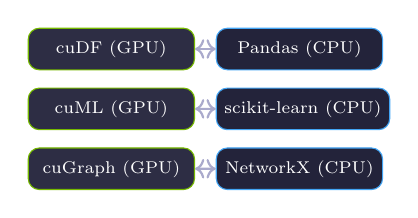
\begin{tikzpicture}[scale=0.88, every node/.style={transform shape},
          r/.style={draw=nvgreen, fill=nvcard, rounded corners=4pt, text=nvwhite, font=\scriptsize, minimum width=2.4cm, minimum height=0.6cm, align=center},
          c/.style={draw=nvblue, fill=nvdarkcard, rounded corners=4pt, text=nvwhite, font=\scriptsize, minimum width=2.4cm, minimum height=0.6cm, align=center}]
        \node[r] (df) {cuDF (GPU)}; \node[c, right=0.3cm of df] (pd) {Pandas (CPU)};
        \node[r, below=0.25cm of df] (ml) {cuML (GPU)}; \node[c, right=0.3cm of ml] (sl) {scikit-learn (CPU)};
        \node[r, below=0.25cm of ml] (g) {cuGraph (GPU)}; \node[c, right=0.3cm of g] (nx) {NetworkX (CPU)};
        \draw[<->,thick,nvgray] (df) -- (pd);
        \draw[<->,thick,nvgray] (ml) -- (sl);
        \draw[<->,thick,nvgray] (g) -- (nx);
      \end{tikzpicture}
      \end{center}
    \end{column}
  \end{columns}
  \certnote{Data Analysis}{Kunci kelulusan ujian: hafalkan pemetaan library di atas. cuDF = Pandas, cuML = scikit-learn, cuGraph = NetworkX.}
\end{frame}

% ── Metrik Performa Statistik ─────────────────────────────
\begin{frame}{Metrik Performa \& Evaluasi}
  \framesubtitle{Bagaimana mengukur keberhasilan model regresi, klasifikasi, dan generasi teks}
  \begin{itemize}\scriptsize
    \item \textbf{Regresi}:
      \begin{itemize}\scriptsize
        \item $R^2$ (Koefisien Determinasi): Proporsi variansi yang dijelaskan model. $R^2 = 0.8$ berarti 80\% variansi terjelaskan.
        \item MSE / RMSE: Menghukum galat (error) besar secara eksponensial. MAE lebih tangguh terhadap pencilan.
      \end{itemize}
    \item \textbf{Klasifikasi}:
      \begin{itemize}\scriptsize
        \item Precision (Ketetapan): Berapa banyak tebakan positif yang benar-benar positif?
        \item Recall (Kepekaan): Berapa banyak kasus positif aktual yang berhasil dideteksi?
        \item F1 Score: Harmonic mean dari Precision dan Recall. Sangat ideal untuk data tidak seimbang (imbalanced data).
      \end{itemize}
    \item \textbf{Generasi Teks NLP (Critical)}:
      \begin{itemize}\scriptsize
        \item \textbf{BLEU}: Kecocokan n-gram output vs referensi; berorientasi \textbf{precision} (mesin terjemahan).
        \item \textbf{ROUGE}: Cakupan n-gram referensi pada output; berorientasi \textbf{recall} (peringkasan).
        \item \textbf{Perplexity}: Tingkat kebingungan model memprediksi kata berikutnya. Semakin kecil nilainya, semakin baik.
      \end{itemize}
  \end{itemize}
  \takeaway{Jangan gunakan Accuracy untuk mengukur LLM generatif; gunakan Perplexity atau metrik berbasis n-gram overlap seperti BLEU/ROUGE.}
\end{frame}

% ============================================================
\acttitle{4}{Domain 3: Experimentation}{Metodologi eksperimen, RAG evaluation, RLHF, dan optimasi inferensi (22\%)}

% ── Desain Eksperimen & Validasi Silang ───────────────────
\begin{frame}{Desain Eksperimen \& Validasi Silang}
  \framesubtitle{Langkah ilmiah untuk mengevaluasi model secara adil dan mencegah kebocoran data}
  \begin{itemize}\footnotesize
    \item \textbf{Prinsip Eksperimen}: Mengontrol variabel (ubah hanya 1 variabel dalam satu waktu), memperbaiki nilai seed acak (random seed) untuk replikasi hasil, dan membuktikan signifikansi secara statistik ($p\text{-value} < 0.05$).
    \item \textbf{Metode Cross-Validation}:
      \begin{itemize}\scriptsize
        \item \textbf{K-Fold}: Membagi data menjadi $K$ bagian secara acak. Latih di $K-1$ bagian, uji di 1 bagian sisa secara bergantian.
        \item \textbf{Stratified K-Fold}: Menjaga distribusi proporsi kelas target pada tiap fold. Wajib untuk klasifikasi data tidak seimbang.
        \item \textbf{Time Series Split}: Memotong data berurutan secara temporal tanpa pengacakan (shuffling) untuk mencegah kebocoran informasi masa depan (\emph{data leakage}).
        \item \textbf{Leave-One-Out (LOO)}: Kasus ekstrem K-Fold di mana $K = N$ (jumlah baris data). Hanya untuk dataset berukuran sangat kecil.
      \end{itemize}
  \end{itemize}
  \takeaway{Mengacak urutan data pada data runtun waktu (*time-series*) adalah kesalahan fatal eksperimen karena memicu kebocoran data masa depan.}
\end{frame}

% ── RAG Evaluation Frameworks ─────────────────────────────
\begin{frame}{Evaluasi Aplikasi RAG}
  \framesubtitle{Mengisolasi kualitas pencarian dokumen dari kualitas generasi teks}
  \begin{columns}[T]
    \begin{column}{0.55\textwidth}
      \begin{itemize}\scriptsize
        \item Sistem RAG dapat gagal di dua tempat: saat \textbf{Retrieval} (salah mencari dokumen) atau saat \textbf{Generation} (salah menulis jawaban).
        \item \textbf{Metrik Kualitas Retrieval}:
          \begin{itemize}\scriptsize
            \item \textbf{Precision@K} / \textbf{Recall@K}: Persentase dokumen relevan pada top-K hasil.
            \item \textbf{MRR} (Mean Reciprocal Rank): Mengukur seberapa cepat dokumen relevan pertama muncul.
          \end{itemize}
        \item \textbf{Metrik Kualitas Generation} (Trilogi RAGAS):
          \begin{itemize}\scriptsize
            \item \textbf{Faithfulness}: Apakah jawaban jujur hanya bersandar pada konteks yang dicari?
            \item \textbf{Answer Relevance}: Apakah jawaban menjawab pertanyaan user?
            \item \textbf{Context Recall}: Apakah retrieval mendapatkan semua informasi yang dibutuhkan?
          \end{itemize}
      \end{itemize}
    \end{column}
    \begin{column}{0.42\textwidth}
      \begin{center}
      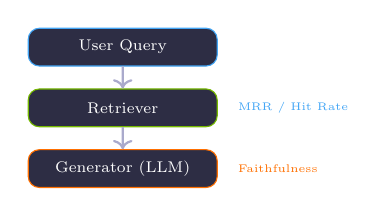
\begin{tikzpicture}[scale=0.8, every node/.style={transform shape},
          box/.style={draw=nvblue, fill=nvcard, rounded corners=4pt, text=nvwhite, font=\scriptsize, minimum width=3cm, minimum height=0.6cm, align=center}]
        \node[box] (q) {User Query};
        \node[box, below=0.35cm of q, draw=nvgreen] (r) {Retriever};
        \node[box, below=0.35cm of r, draw=nvorange] (g) {Generator (LLM)};
        \draw[->,thick,nvgray] (q) -- (r);
        \draw[->,thick,nvgray] (r) -- (g);
        \node[text=nvblue, font=\tiny, right=0.2cm of r] {MRR / Hit Rate};
        \node[text=nvorange, font=\tiny, right=0.2cm of g] {Faithfulness};
      \end{tikzpicture}
      \end{center}
    \end{column}
  \end{columns}
  \certnote{Experimentation}{Groundedness / Faithfulness mengevaluasi adanya halusinasi model dengan membandingkan teks output LLM langsung terhadap dokumen konteks.}
\end{frame}

% ── RLHF & Penyelarasan Model ────────────────────────────
\begin{frame}{RLHF \& Penyelarasan Model}
  \framesubtitle{Menyelaraskan perilaku LLM generatif dengan nilai-nilai dan preferensi manusia}
  \begin{columns}[T]
    \begin{column}{0.6\textwidth}
      \begin{itemize}\scriptsize
        \item \textbf{Tujuan}: Model tidak hanya pintar merangkai kata, tapi juga aman, membantu (\emph{helpful}), dan jujur (\emph{honest}).
        \item \textbf{Tiga Tahap Klasik RLHF}:
          \begin{enumerate}\scriptsize
            \item \textbf{SFT} (Supervised Fine-Tuning): Melatih model dasar menggunakan sepasang data instruksi-respon berkualitas tinggi.
            \item \textbf{Reward Model Training}: Melatih model terpisah untuk menebak skor kesukaan manusia dari beberapa alternatif jawaban LLM.
            \item \textbf{RL Fine-Tuning} (PPO): Mengoptimalkan model SFT via RL memakai skor Reward Model, plus penalty KL agar model tidak rusak.
          \end{enumerate}
        \item \textbf{DPO} (Direct Preference Optimization): Metode modern yang langsung melatih model pada data preferensi tanpa perlu membuat Reward Model terpisah.
      \end{itemize}
    \end{column}
    \begin{column}{0.36\textwidth}
      \begin{center}
      \begin{beamercolorbox}[rounded=true,shadow=false,sep=8pt]{block body}
        {\footnotesize\color{nvlightgreen}\textbf{Alternatif Alignment:}}
        \vspace{0.3em}
        {\scriptsize\color{nvwhite}
        $\bullet$ \textbf{RLAIF}: Menggunakan umpan balik AI (bukan manusia) untuk melatih reward model.\\
        $\bullet$ \textbf{Constitutional AI}: Model mengoreksi perilakunya sendiri berdasarkan prinsip etika tertulis (konstitusi).}
      \end{beamercolorbox}
      \end{center}
    \end{column}
  \end{columns}
  \takeaway{PPO menggunakan algoritma reinforcement learning yang rumit, sedangkan DPO menyederhanakannya menjadi optimasi fungsi loss klasifikasi biner biasa.}
\end{frame}

% ── Optimasi Inferensi ───────────────────────────────────
\begin{frame}{Metode Optimasi Inferensi}
  \framesubtitle{Teknik mempercepat throughput dan memangkas kebutuhan memori GPU di fase produksi}
  \begin{columns}[T]
    \begin{column}{0.54\textwidth}
      \begin{itemize}\footnotesize
        \item \textbf{Quantization}: Menurunkan presisi angka bobot model (FP32 $\to$ FP16 $\to$ INT8 $\to$ INT4):
          \begin{itemize}\scriptsize
            \item \textbf{PTQ} (Post-Training Quantization): Konversi langsung setelah model selesai dilatih. Cepat, namun ada risiko penurunan akurasi pada bit sangat rendah.
            \item \textbf{QAT} (Quantization-Aware Training): Mensimulasikan efek kuantisasi saat latihan. Akurasi terjaga lebih baik.
          \end{itemize}
        \item \textbf{Pruning}: Memotong bobot atau neuron yang tidak berkontribusi signifikan pada performa model.
        \item \textbf{Distillation}: Melatih model kecil (student) untuk meniru distribusi probabilitas model besar (teacher).
      \end{itemize}
    \end{column}
    \begin{column}{0.42\textwidth}
      \begin{center}
      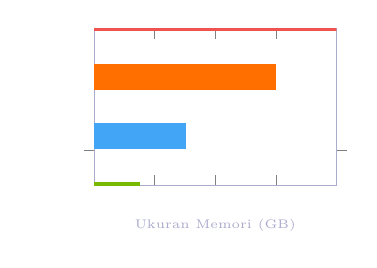
\begin{tikzpicture}[scale=0.9, every node/.style={transform shape}]
        \begin{axis}[
          width=5cm, height=3.8cm,
          xbar, xmin=0, xmax=4,
          axis line style={nvgray}, tick label style={nvwhite, font=\tiny},
          xlabel={\color{nvgray}\tiny Ukuran Memori (GB)},
          symbolic y coords={INT4, INT8, FP16, FP32}, ytick=data,
          nodes near coords, nodes near coords style={nvwhite, font=\tiny},
          enlarge y limits=0.4, bar width=10pt]
          \addplot[fill=nvgreen, draw=nvgreen] coordinates {(0.75,INT4)};
          \addplot[fill=nvblue, draw=nvblue] coordinates {(1.5,INT8)};
          \addplot[fill=nvorange, draw=nvorange] coordinates {(3.0,FP16)};
          \addplot[fill=nvred, draw=nvred] coordinates {(6.0,FP32)};
        \end{axis}
      \end{tikzpicture}
      \end{center}
    \end{column}
  \end{columns}
  \certnote{Experimentation}{Kuantisasi INT4 memangkas ukuran model secara drastis ($\sim$8x lebih kecil dibanding FP32), memungkinkannya muat di GPU kelas konsumen.}
\end{frame}

% ============================================================
\acttitle{5}{Domain 4: Software Development}{Aplikasi Python NLP, Triton, TensorRT, NeMo, dan distributed training (24\%)}

% ── Python NLP Packages: spaCy & NumPy ───────────────────
\begin{frame}{Library NLP Python: spaCy \& NumPy}
  \framesubtitle{Kolaborasi pemrosesan teks linguistik cepat dengan komputasi matriks cepat}
  \begin{columns}[T]
    \begin{column}{0.54\textwidth}
      \begin{itemize}\small
        \item \textbf{spaCy}: Desain khusus untuk industri (cepat, siap produksi).
          \begin{itemize}\scriptsize
            \item Objek inti: \textbf{Doc} (dokumen terproses), \textbf{Token} (kata/tanda baca), \textbf{Span} (irisan Doc/frasa).
            \item Pipeline: Tokenizer $\to$ Tagger $\to$ Parser $\to$ NER.
          \end{itemize}
        \item \textbf{NumPy}: Komputasi matriks/array berkinerja tinggi.
          \begin{itemize}\scriptsize
            \item Mempercepat pencarian kesamaan kosinus (*cosine similarity*) via operasi vektor terakselerasi.
            \item Mendukung *broadcasting* (operasi elemen-wise pada dimensi array yang berbeda).
          \end{itemize}
      \end{itemize}
    \end{column}
    \begin{column}{0.42\textwidth}
      \begin{center}
      \begin{beamercolorbox}[rounded=true,shadow=false,sep=8pt]{block body}
        {\footnotesize\color{nvlightgreen}\textbf{Pola Kolaborasi:}}
        \vspace{0.3em}
        {\scriptsize\color{nvwhite}
        1. Gunakan \textbf{spaCy} untuk mem-parsing teks linguistik dan mengekstrak vektor kata.\\
        2. Tumpuk (\emph{stack}) vektor tersebut ke dalam array \textbf{NumPy} menggunakan \texttt{np.vstack()}.\\
        3. Lakukan kalkulasi kesamaan matriks cepat di \textbf{NumPy}.}
      \end{beamercolorbox}
      \end{center}
    \end{column}
  \end{columns}
  \takeaway{spaCy berfokus pada analisis bahasa (linguistik), sedangkan NumPy berfokus pada matematika array linier di balik kata tersebut.}
\end{frame}

% ── NVIDIA Deployment Stack: Triton Inference Server ──────
\begin{frame}{NVIDIA Serving Stack: Triton Server}
  \framesubtitle{Mesin penyaji model handal dengan dynamic batching \& multi-framework support}
  \begin{columns}[T]
    \begin{column}{0.54\textwidth}
      \begin{itemize}\footnotesize
        \item \textbf{Triton Inference Server} menyajikan model ke production dengan latensi rendah dan throughput tinggi.
        \item \textbf{Multi-Framework}: Menjalankan model PyTorch, TensorFlow, ONNX, dan TensorRT secara bersamaan.
        \item \textbf{Dynamic Batching}: Menggabungkan beberapa request inferensi tunggal dari pengguna yang berbeda menjadi satu batch besar di GPU secara otomatis.
        \item \textbf{Struktur Model Repository (Wajib)}:
          \begin{itemize}\scriptsize
            \item Harus memuat file \texttt{config.pbtxt} untuk mendefinisikan tipe input/output tensor, ukuran dimensi, dan model backend.
          \end{itemize}
      \end{itemize}
    \end{column}
    \begin{column}{0.42\textwidth}
      \begin{center}
      \begin{tikzpicture}[scale=0.8, every node/.style={transform shape},
          folder/.style={draw=nvblue, fill=nvdarkcard, font=\scriptsize\ttfamily, minimum width=2.5cm, minimum height=0.5cm, align=left}]
        \node[folder] (root) {model\_repository/};
        \node[folder, below=0.25cm of root, xshift=0.5cm] (name) {└── model\_name/};
        \node[folder, below=0.2cm of name, xshift=0.5cm] (cfg) {├── config.pbtxt};
        \node[folder, below=0.2cm of cfg] (v) {└── 1/};
        \node[folder, below=0.2cm of v, xshift=0.5cm] (model) {└── model.onnx};
        \draw[-,thick,nvgray] (root) |- (name);
        \draw[-,thick,nvgray] (name) |- (cfg);
        \draw[-,thick,nvgray] (name) |- (v);
        \draw[-,thick,nvgray] (v) |- (model);
      \end{tikzpicture}
      \end{center}
    \end{column}
  \end{columns}
  \certnote{Software Development}{Hafalkan struktur direktori Triton di atas. Salah menaruh file config.pbtxt atau subfolder versi (1/) akan membuat model gagal dimuat.}
\end{frame}

% ── TensorRT & TensorRT-LLM ──────────────────────────────
\begin{frame}{Optimasi dengan TensorRT \& TensorRT-LLM}
  \framesubtitle{Compiler khusus GPU NVIDIA untuk merombak grafik jaringan saraf tiruan}
  \begin{columns}[T]
    \begin{column}{0.54\textwidth}
      \begin{itemize}\footnotesize
        \item \textbf{TensorRT} merestrukturisasi model dengan:
          \begin{itemize}\scriptsize
            \item \emph{Layer \& Tensor Fusion}: Menggabungkan layer operasi matematika yang terpisah menjadi satu instruksi GPU (\emph{kernel}).
            \item \emph{Kernel Auto-Tuning}: Memilih algoritma komputasi tercepat yang sesuai dengan tipe GPU spesifik target.
          \end{itemize}
        \item \textbf{TensorRT-LLM} (Optimal untuk model bahasa besar):
          \begin{itemize}\scriptsize
            \item \textbf{Paged KV-Cache}: Memecah memori kunci-nilai attention menjadi halaman diskrit untuk mencegah fragmentasi VRAM.
            \item \textbf{In-Flight Batching}: Memasukkan request baru ke GPU tanpa menunggu proses generasi request sebelumnya selesai.
          \end{itemize}
      \end{itemize}
    \end{column}
    \begin{column}{0.42\textwidth}
      \begin{center}
      \begin{beamercolorbox}[rounded=true,shadow=false,sep=8pt]{block body}
        {\footnotesize\color{nvlightgreen}\textbf{Alur Ekspor TRT:}}
        \vspace{0.3em}
        {\scriptsize\color{nvwhite}
        PyTorch (.pt) $\to$ Ekspor ke \textbf{ONNX} (Grafik Umum) $\to$ Dikompilasi oleh \textbf{TensorRT} menjadi Engine (.plan) terikat arsitektur GPU target.}
      \end{beamercolorbox}
      \end{center}
    \end{column}
  \end{columns}
  \takeaway{Engine (.plan) hasil kompilasi TensorRT tidak portabel --- ia dibuat khusus dan hanya bisa jalan di arsitektur GPU yang sama saat proses kompilasi.}
\end{frame}

% ── NVIDIA NeMo Framework ─────────────────────────────────
\begin{frame}{NVIDIA NeMo Framework}
  \framesubtitle{Platform komprehensif pelatihan, adaptasi, dan penyelarasan model bahasa besar}
  \begin{columns}[T]
    \begin{column}{0.55\textwidth}
      \begin{itemize}\small
        \item \textbf{NeMo} menyediakan koleksi modul teroptimasi untuk pembuatan Conversational AI, Speech, dan Generative LLM.
        \item \textbf{NeMo LLM}: Menyediakan framework pelatihan model skala masif berbasis Megatron.
        \item \textbf{Pilihan Fine-Tuning (Adaptasi)}:
          \begin{itemize}\scriptsize
            \item \emph{PEFT (Parameter-Efficient Fine-Tuning)}: Mengurangi memori latihan secara ekstrem.
            \item \emph{LoRA}: Menyisipkan matriks dekomposisi rank rendah ke lapisan attention.
            \item \emph{P-Tuning}: Mempelajari representasi virtual prompt secara kontinu di embedding layer.
          \end{itemize}
      \end{itemize}
    \end{column}
    \begin{column}{0.42\textwidth}
      \begin{center}
      \begin{beamercolorbox}[rounded=true,shadow=false,sep=8pt]{block body}
        {\footnotesize\color{nvblue}\textbf{NeMo Collections:}}
        \vspace{0.3em}
        {\scriptsize\color{nvwhite}
        $\bullet$ \textbf{NeMo LLM} (Generative AI)\\
        $\bullet$ \textbf{NeMo Guardrails} (Safety / Topical)\\
        $\bullet$ \textbf{NeMo ASR} (Speech-to-Text Conformer)\\
        $\bullet$ \textbf{NeMo TTS} (Text-to-Speech FastPitch)}
      \end{beamercolorbox}
      \end{center}
    \end{column}
  \end{columns}
  \takeaway{NeMo mengintegrasikan semua kebutuhan siklus hidup model LLM dari pra-pemrosesan data, pemetaan paralel, hingga pagar keamanan runtime.}
\end{frame}

% ── Distributed Training & Scaling Laws ───────────────────
\begin{frame}{Distributed Training \& Scaling Laws}
  \framesubtitle{Mengkoordinasikan multi-GPU untuk melatih model raksasa secara efisien}
  \begin{columns}[T]
    \begin{column}{0.56\textwidth}
      \begin{itemize}\footnotesize
        \item \textbf{NCCL} (NVIDIA Collective Communications Library): Library komunikasi antar GPU berkecepatan tinggi (melalui NVLink/NVSwitch).
        \item \textbf{AllReduce (Ring AllReduce)}: Protokol pembagian gradien di mana GPU terhubung melingkar. Komunikasi data tidak terpengaruh jumlah GPU.
        \item \textbf{Data Parallelism} vs \textbf{Model Parallelism}: Data paralel membagi batch data (model disalin penuh ke tiap GPU). Model paralel membagi layer model karena tidak muat di satu GPU.
        \item \textbf{Chinchilla Scaling Laws}: Untuk latihan komputasi optimal, parameter model dan jumlah token data harus tumbuh seimbang (skala 1:1). Model 70B butuh $\sim$1.4 Triliun token.
      \end{itemize}
    \end{column}
    \begin{column}{0.4\textwidth}
      \begin{center}
      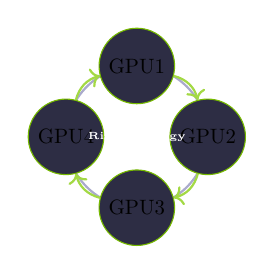
\begin{tikzpicture}[scale=0.75, every node/.style={transform shape}]
        \draw[nvgray, thick] (0,0) circle (1.2cm);
        \node[draw=nvgreen, fill=nvcard, circle, minimum size=0.8cm] (g1) at (0,1.2) {GPU1};
        \node[draw=nvgreen, fill=nvcard, circle, minimum size=0.8cm] (g2) at (1.2,0) {GPU2};
        \node[draw=nvgreen, fill=nvcard, circle, minimum size=0.8cm] (g3) at (0,-1.2) {GPU3};
        \node[draw=nvgreen, fill=nvcard, circle, minimum size=0.8cm] (g4) at (-1.2,0) {GPU4};
        \draw[->,thick,nvlightgreen] (g1) to[bend left] (g2);
        \draw[->,thick,nvlightgreen] (g2) to[bend left] (g3);
        \draw[->,thick,nvlightgreen] (g3) to[bend left] (g4);
        \draw[->,thick,nvlightgreen] (g4) to[bend left] (g1);
        \node[font=\tiny\bfseries, text=nvwhite] at (0,0) {Ring topology};
      \end{tikzpicture}
      \end{center}
    \end{column}
  \end{columns}
  \certnote{Software Development}{Pahami hardware GPU NVIDIA (H100 untuk enterprise training/inference, L40S untuk visual/inference, T4 16GB untuk server irit).}
\end{frame}

% ============================================================
\acttitle{6}{Domain 5: Trustworthy AI}{Kepatuhan etika kecerdasan buatan, privasi data pengguna, dan pagar pengaman (10\%)}

% ── Enam Pilar Trustworthy AI ─────────────────────────────
\begin{frame}{Enam Pilar Trustworthy AI}
  \framesubtitle{Kerangka evaluasi kualitas non-fungsional sistem kecerdasan buatan}
  \begin{center}
  \renewcommand{\arraystretch}{1.0}{\footnotesize\setlength{\tabcolsep}{6pt}
  \begin{tabular}{@{}p{0.18\linewidth}p{0.50\linewidth}p{0.24\linewidth}@{}}
    \toprule \rowcolor{nvcard!50}
    \textbf{Pilar Utama} & \textbf{Tujuan \& Definisi} & \textbf{Penerapan di LLM} \\ \midrule
    \textbf{1. Fairness} & Menghindari bias dan diskriminasi hasil antar kelompok. & Demographic parity \& equal odds \\
    \textbf{2. Transparency} & Sistem terbuka, terdokumentasi, dan dapat dimengerti. & Pembuatan Model Cards \\
    \textbf{3. Privacy} & Perlindungan data sensitif dan kepatuhan konsensual. & PII Masking \& UU-PDP/GDPR \\
    \textbf{4. Safety} & Sistem tidak membahayakan pengguna atau lingkungan. & Detoksifikasi konten toksik \\
    \textbf{5. Accountability} & Kejelasan tanggung jawab hukum dan jejak audit keputusan. & Logging rails aktif di API \\
    \textbf{6. Robustness} & Daya tahan terhadap kegagalan dan serangan musuh. & Pertahanan jailbreak \\
    \bottomrule
  \end{tabular}}
  \end{center}
  \takeaway{Trustworthy AI wajib jadi arsitektur sistem di produksi --- bukan sekadar konsep etika teoritis.}
\end{frame}

% ── Data Privacy & UU-PDP ─────────────────────────────────
\begin{frame}{Privasi Data \& Regulasi UU-PDP}
  \framesubtitle{Implementasi kepatuhan hukum pelindungan data pada arsitektur LLM}
  \begin{columns}[T]
    \begin{column}{0.54\textwidth}
      \begin{itemize}\scriptsize
        \item \textbf{Data Minimization}: Hanya kirim informasi yang benar-benar dibutuhkan ke LLM (cegah kebocoran).
        \item \textbf{PII Masking} (Data Anonymization): Mengganti data sensitif (NIK, nomor rekening, nomor HP) dengan placeholder sebelum dikirim ke LLM / disimpan ke log.
        \item \textbf{UU PDP No. 27/2022}:
          \begin{itemize}\scriptsize
            \item Melanggar privasi pengguna dapat dikenakan denda hingga \textbf{2\% dari pendapatan tahunan}.
            \item Kebocoran data wajib dilaporkan maksimal \textbf{72 jam} sejak terdeteksi.
          \end{itemize}
      \end{itemize}
    \end{column}
    \begin{column}{0.42\textwidth}
      \begin{center}
      \begin{beamercolorbox}[rounded=true,shadow=false,sep=5pt]{block body}
        {\footnotesize\color{nvblue}\textbf{Penyelamatan Privasi:}}
        \vspace{0.1em}
        {\scriptsize\color{nvwhite}
        $\bullet$ \textbf{Differential Privacy}: Menambahkan derau acak (\emph{noise}) pada data/query agar data individu tidak bisa di-reverse.\\
        $\bullet$ \textbf{Federated Learning}: Melatih model pada perangkat lokal masing-masing tanpa mengumpulkan data mentah ke server pusat.}
      \end{beamercolorbox}
      \end{center}
    \end{column}
  \end{columns}
  \takeaway{Masking data pribadi (PII) menggunakan kombinasi regex presisi adalah langkah wajib sebelum data menyentuh runtime LLM.}
\end{frame}

% ── NeMo Guardrails & Morpheus ────────────────────────────
\begin{frame}{Penerapan Pagar Keamanan Runtime}
  \framesubtitle{Membangun pos pemeriksaan keamanan input dan output model LLM}
  \begin{columns}[T]
    \begin{column}{0.55\textwidth}
      \begin{itemize}\footnotesize
        \item \textbf{NeMo Guardrails} membuat sistem kendali dialog terprogram menggunakan bahasa \textbf{Colang}:
          \begin{itemize}\scriptsize
            \item \emph{Topical Rails}: Menjaga LLM agar tidak keluar dari topik bisnis (off-topic blocker).
            \item \emph{Safety Rails}: Mendeteksi respon berbahaya, kasar, atau melanggar hukum.
            \item \emph{Jailbreak Detection}: Memblokir rekayasa prompt jahat yang memaksa LLM melewati filter keselamatan.
          \end{itemize}
        \item \textbf{NVIDIA Morpheus}: Framework AI khusus keamanan siber untuk mendeteksi ancaman anomali data pipeline secara real-time.
        \item \textbf{Model Explainability}: SHAP dan LIME untuk menerjemahkan kontribusi fitur di balik keputusan AI.
      \end{itemize}
    \end{column}
    \begin{column}{0.41\textwidth}
      \begin{center}
      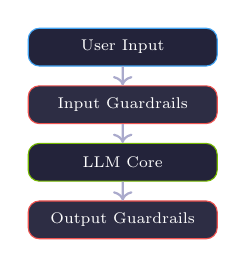
\begin{tikzpicture}[scale=0.8, every node/.style={transform shape},
          r/.style={draw=nvred, fill=nvcard, rounded corners=4pt, text=nvwhite, font=\scriptsize, minimum width=3cm, minimum height=0.6cm, align=center}]
        \node[draw=nvblue, fill=nvdarkcard, rounded corners=4pt, text=nvwhite, font=\scriptsize, minimum width=3cm, minimum height=0.6cm] (in) {User Input};
        \node[r, below=0.3cm of in] (rail) {Input Guardrails};
        \node[draw=nvgreen, fill=nvdarkcard, rounded corners=4pt, text=nvwhite, font=\scriptsize, minimum width=3cm, minimum height=0.6cm, below=0.3cm of rail] (llm) {LLM Core};
        \node[r, below=0.3cm of llm] (orail) {Output Guardrails};
        \draw[->,thick,nvgray] (in) -- (rail);
        \draw[->,thick,nvgray] (rail) -- (llm);
        \draw[->,thick,nvgray] (llm) -- (orail);
      \end{tikzpicture}
      \end{center}
    \end{column}
  \end{columns}
  \takeaway{Pagar keamanan harus dipasang dua arah: menyaring bahaya dari *Input* user, dan memvalidasi kebenaran *Output* LLM.}
\end{frame}

% ============================================================
\acttitle{7}{Strategi Belajar \& Tips Lulus}{Persiapan jadwal, simulasi ujian, dan teknik menjawab soal secara efektif}

% ── Sumber Belajar Resmi NVIDIA DLI ───────────────────────
\begin{frame}{Sumber Belajar Resmi: Kursus NVIDIA DLI}
  \framesubtitle{Blueprint resmi memetakan tiap domain ke kursus Deep Learning Institute (DLI)}
  \begin{center}
  \renewcommand{\arraystretch}{1.25}{\footnotesize\setlength{\tabcolsep}{6pt}
  \begin{tabular}{@{}p{0.32\linewidth}p{0.60\linewidth}@{}}
    \toprule \rowcolor{nvcard!50}
    \textbf{Domain (Bobot)} & \textbf{Kursus DLI yang Dipetakan} \\ \midrule
    Core ML/AI (30\%) & Getting Started With Deep Learning $\cdot$ Fundamentals of Deep Learning \\
    Software Dev (24\%) & Introduction to / Building Transformer-Based NLP Applications \\
    Experimentation (22\%) & Building LLM Applications with Prompt Engineering \\
    Data Analysis (14\%) & Accelerating End-to-End Data Science Workflows (RAPIDS) \\
    Trustworthy AI (10\%) & Rapid Application Development With LLMs \\
    \bottomrule
  \end{tabular}}
  \end{center}
  \certnote{Catatan}{Kursus DLI berbayar (mulai \$90 self-paced, \$500 workshop). Materi bootcamp Navasena (Modul 01--06) sudah memetakan kelima domain ini sebagai persiapan gratis.}
\end{frame}

% ── Jadwal Persiapan Belajar ──────────────────────────────
\begin{frame}{Jadwal Persiapan Belajar}
  \framesubtitle{Rekomendasi alokasi waktu 8--12 minggu menuju hari ujian}
  \begin{center}
  \renewcommand{\arraystretch}{1.2}{\footnotesize\setlength{\tabcolsep}{8pt}
  \begin{tabular}{@{}p{0.20\linewidth}p{0.50\linewidth}p{0.20\linewidth}@{}}
    \toprule \rowcolor{nvcard!50}
    \textbf{Fase Latihan} & \textbf{Topik Fokus Utama} & \textbf{Alokasi Waktu} \\ \midrule
    \textbf{Minggu 1--2} & Memetakan blueprint objektif ujian & 5 jam / minggu \\
    \textbf{Minggu 3--6} & Pendalaman teori arsitektur LLM & 10--15 jam / minggu \\
    \textbf{Minggu 7--8} & Simulasi tes mandiri & 15 jam / minggu \\
    \textbf{Minggu 9--10} & Evaluasi hasil simulasi & 15 jam / minggu \\
    \textbf{Minggu 11--12} & Review ringkasan & 10 jam / minggu \\
    \bottomrule
  \end{tabular}}
  \end{center}
  \takeaway{Prioritaskan belajar pada domain dengan bobot nilai tertinggi: Core ML/AI (30\%) dan Software Development (24\%).}
\end{frame}

% ── Taktik Menjawab Soal ──────────────────────────────────
\begin{frame}{Taktik Menjawab Soal Ujian}
  \framesubtitle{Tips memaksimalkan skor saat menghadapi soal pilihan ganda di portal ujian}
  \begin{itemize}\small
    \item \textbf{Metode Eliminasi}: Buang pilihan jawaban yang jelas-jelas salah terlebih dahulu (membantu menaikkan probabilitas kebenaran tebakan).
    \item \textbf{Perhatikan Kata Kunci Negatif}: Waspadai kata seperti ``\emph{NOT}'', ``\emph{EXCEPT}'', atau ``\emph{UNLESS}'' yang dapat menjebak pembaca yang terburu-buru.
    \item \textbf{Jangan Kosongkan Jawaban}: Tidak ada sistem penalti (nilai minus) untuk tebakan yang salah. Jawab semua soal!
    \item \textbf{Gunakan Intuisi Pertama}: Umumnya, jawaban yang terlintas pertama kali di pikiran adalah tebakan yang paling akurat. Jangan mengubah jawaban berulang kali kecuali Anda benar-benar yakin.
  \end{itemize}
  \takeaway{Rata-rata Anda memiliki waktu $\sim$60--72 detik per soal. Jangan membuang waktu lebih dari 2 menit pada satu soal yang rumit.}
\end{frame}

% ── Kesimpulan & Penutup ──────────────────────────────────
\begin{frame}{Kesimpulan \& Penutup}
  \framesubtitle{Langkah berikutnya menuju kelulusan sertifikasi NVIDIA NCA-GENL}
  \begin{columns}[T]
    \begin{column}{0.54\textwidth}
      \begin{itemize}\small
        \item Sertifikasi NCA-GENL membuktikan pemahaman teori dasar kecerdasan buatan sekaligus implementasi praktis di ekosistem NVIDIA.
        \item Latihan coding menggunakan library cuDF, spaCy, dan deployment Triton server sangat membantu pemahaman konseptual.
        \item Jaga kesehatan, istirahat cukup sebelum hari ujian, dan pastikan koneksi internet \& webcam lancar.
      \end{itemize}
    \end{column}
    \begin{column}{0.42\textwidth}
      \begin{center}
      \begin{beamercolorbox}[rounded=true,shadow=false,sep=8pt]{block body}
        {\color{nvgreen}\Large\bfseries Semoga Sukses! 🚀}
        \vspace{0.5em}
        {\scriptsize\color{nvwhite}
        Dengan persiapan matang bersama materi Navasena, Anda siap meraih sertifikat resmi NVIDIA Certified Associate!}
      \end{beamercolorbox}
      \end{center}
    \end{column}
  \end{columns}
  \takeaway{Semoga berhasil dalam perjalanan belajar Anda. Sampai jumpa di jajaran profesional AI bersertifikasi!}
\end{frame}

\end{document}
